\section{Flavour Physics}
%
We still need a theory of the quark masses (and mixing). The third generation in the standard model consists of:
\begin{itemize}
\item \textbf{$\tau$ lepton: } discovered in 1975 at SLAC, with a mass $m_\tau = $ 1.78 GeV. This was relatively unexpected;
\item \textbf{$b$ quark: } discovered in 1977 at Fermilab, with a mass $m_b$ = 5 GeV. Seen in the form of the $\Upsilon = b\bar{b}$ particle with mass 10 GeV;
\item \textbf{$\nu_\tau$ neutrino: } finally seen in 2000 at Fermilab. This was very difficult!;
\item \textbf{$t$ quark: } finally discovered in 1995 at the Tevatron, Fermilab, with a mass $m_t$ = 175 GeV.
\end{itemize}
The top quark is very heavy: $m_t > m_W, m_Z, m_h$, and decays very quickly via $t \to Wb$ before it can hadronise. Because of anomalies it does not decouple from low energy processes; its involvement is needed for consistency.

There are only three generations (3 light neutrinos).
%
\subsection{The Quark Masses}
%
As with leptons, these must arise through Yukawa interactions. We have left-handed doublets and right-handed singlets under SU(2)$_L$:
\[ Q_L^i = \left( \begin{array}{cc}
u_L   \\
d_L  \end{array} \right), \qquad
\left( \begin{array}{cc}
c_L   \\
s_L   \end{array} \right), \qquad
\left( \begin{array}{cc}
t_L   \\
b_L   \end{array} \right);\]
\[ 
u_R^i = \qquad u_R, \qquad c_R, \qquad t_R, \qquad;
\]
\[ 
d_R^i = \qquad d^\prime_R, \qquad s^\prime_R, \qquad b_R, \qquad \text{for } i=1,2,3.
\]
where the "up-type" quarks appear on the top row and "down-type" quarks on the bottom row. For leptons we introduced Yukawa coupling to a complex doublet
\[\phi = \left( \begin{array}{cc}
\phi^+ \\
\phi^0 \end{array} \right),
\]
which can give mass to the down-type quarks through $<\phi^0> = v$. What about up-type quarks? Consider the conjugate field
\[
\phi^c \equiv (i\sigma_2)\phi^+ = \left( \begin{array}{cc}
0 & 1   \\
-1 & 0  \end{array} \right) 
\left( \begin{array}{cc}
\phi^{+ *}   \\
\phi^{0 *}  \end{array} \right) = 
\left( \begin{array}{cc}
\phi^{0 *}   \\
-\phi^{+ *}  \end{array} \right).
\]
Clearly $\phi^c$ has $Y = - \frac{1}{2}$. Moreover
\begin{equation}
(i\sigma_2)\sigma_i^* = -\sigma_i(i\sigma_2),
\end{equation}
so under SU(2)$_L$, $\phi \to U \phi = \exp(\frac{i}{2}\underline{\alpha}\cdot \underline{\sigma})$, and
\begin{equation}
\phi^c \to (i\sigma_2)e^{-\frac{i}{2}\underline{\alpha}\cdot\underline{\sigma}^*} \phi^* = e^{+\frac{i}{2}\underline{\alpha}\cdot{\sigma}}(i\sigma_2)\phi^* = U \phi^c,
\end{equation}
so $\phi^c$ is also a doublet under SU(2)$_L$.

Note that this works because SU(2) is "pseudoreal". This implies also that $tr \sigma_i \{\sigma_j, \sigma_k \} = 0$, i.e. it is anomaly free. This does not generalise to SU(N), for N>2: for this we would need a second Higgs doublet. So besides $\bar{Q}_L\phi d_R$, which gives mass to down-type quarks, we also have $\bar{Q}_L\phi^c u_R$, which gives mass to up-type quarks. (What does the missing line here say?)

So the most general Yukawa term for quarks is
\begin{equation}
\mathcal{L}_{Y} = -(Y_{ij}^d \bar{Q}_L^i \phi d_R^j + h.c.) - (Y_{ij}^u \bar{Q}_L^i \phi^c u_R^j + h.c.),
\end{equation}
where $Y^u$, $Y^d$ are two arbitrary 3$\times$3 matrices. After spontaneous symmetry breaking
\begin{equation}
\phi \to \frac{v}{\sqrt{2}}\begin{pmatrix} 0 \\ 1 \end{pmatrix},
\qquad \phi^c \to \frac{v}{\sqrt{2}}\begin{pmatrix} 1 \\ 0 \end{pmatrix}.
\end{equation}
So defining mass matrices $M_{ij}^u = \frac{v}{\sqrt{2}}Y_{ij}^u$; $M_{ij}^d = \frac{v}{\sqrt{2}}Y_{ij}^d$, we have
\begin{equation}
\mathcal{L}_{Y} = -(M_{ij}^u \bar{u}_L^i u_R^j + h.c.) - (M_{ij}^d \bar{d}_L^i d_R^j + h.c.).
\end{equation}
Note that there is mixing between up-type quarks and between down-type quarks, but not between different types: this would violate U(1)$_Y$. We need to diagonalise the mass matrices, in order to find the "mass basis". Consider $M^u$: $M^{u \dagger} M^u$ is hermitian, so the real positive eigenvalues are $m_u^2$, $m_c^2$ and $m_t^2$. Similarly, $M^{d \dagger} M^d$ is hermitian, so the real positive eigenvalues are $m_d^2$, $m_s^2$ and $m_b^2$.
\subsubsection{Lemma: $\exists$ unitary matrices $L$ and $R$ such that $LMR^\dagger=D$, a diagonal matrix with masses $m_u^2$, $m_c^2$ and $m_t^2$ (or $m_d$, $m_s^2$ and $m_b^2$).}
\textbf{Proof: }
\begin{equation}
(M^\dagger M)^\dagger = M^\dagger M, 
\end{equation}
so $\exists$ a unitary matrix $R$ such that
\begin{equation}
R^\dagger(M^\dagger M)R = D^2,
\end{equation}
where $D$ is a diagonal matrix with real, positive eigenvalues. Then define $L = MRD^{-1}$, so
\begin{equation}
L^\dagger = D^{-1}R^\dagger M^\dagger, \qquad L^\dagger L = D^{-1}R^\dagger M^\dagger MR D^{-1} = 1,
\end{equation}
i.e. $L$ is unitary and $L^\dagger MR = D^{-1}R^\dagger M^\dagger MR = D$, so we have
\begin{equation}
L^{u \dagger}M^u R^u = D^u, \qquad L^{d \dagger}M^d R^d = D^d,
\end{equation}
and if we let
\begin{equation}
\begin{split}
u_R \to R^u u_R \qquad u_L \to L^u u_L \\
d_R \to R^d d_R \qquad d_L \to L^d d_L
\end{split}
\end{equation}
then the mass terms become diagonal:
\begin{equation}
- \sum_{q = u,c,t} m_q(\bar{q}_L q_R + \bar{q}_R q_L) - \sum_{q = d,s,b} m_q(\bar{q}_L q_R + \bar{q}_R q_L) = - \sum_{q=u,c,t,d,s,b} m_q \bar{q}{q}.
\end{equation}
It is easy to see that the kinetic term remains diagonal:
\begin{equation}
\mathcal{L}_{D,\ kin} = \sum_{q = d,s,b}(\bar{q}_L i \slashed{\partial} q_L + \bar{q}_R i \slashed{\partial} q_R),
\end{equation}
and $L^u$, $L^d$, $R^u$, $R^d$ are all hermitian. Likewise, the quark contribution to the neutral current
\begin{equation}
J_\mu^{NC} = \sum_{q=u,c,t}\bar{q}\gamma_\mu\bigg(\frac{-4}{3}\sin^2\theta_w +\frac{1}{2}(1-\gamma^5)\bigg)q + \sum_{q=d,s,b}\bar{q}\gamma_\mu\bigg(\frac{2}{3}\sin^2\theta_w -\frac{1}{2}(1-\gamma^5)\bigg)q,
\end{equation}
is invariant, since 
\begin{equation}
\bar{q}\gamma^\mu q = \bar{q}_L\gamma^\mu q_L + \bar{q}_L\gamma^\mu q_R.
\end{equation}
This is the GIM mechanism, which we saw earlier in the course.
%
\subsection{The CKM Matrix}
%
Charge conjugation relates up-type quarks to down-type quarks, so 
\begin{equation}
\begin{split}
\frac{1}{2} J_\mu^h = \sum_i \bar{u}_L^i \gamma_\mu d_L^i &\to \sum_{ijk} \bar{u}_L^i(L^{u \dagger})^{ij}\gamma_\mu(L^{d})^{jk}d_L^k \\
&\equiv \sum_{ij} \bar{u}_L^i \gamma_\mu V^{ij} d_L^j,
\end{split}
\end{equation}
where $V = L^{u \dagger} L^d$ is the CKM matrix, named after Cabibbo, Kobayashi and Maskawa (1973). The CKM matrix mixes the charged current interactions.

$V$ is unitary: $V^\dagger V = L^{d \dagger}L^u L^{u \dagger} L^d = 1$. There are $N$ generations, so $V$ is an $N\times N$ complex matrix and has $2N^2$ real parameters. Unitarity gives $N^2$ constraints, so there are $N^2$ remaining real parameters. However, phase changes of the form $u_L^i \to \exp(i\alpha_i)u_L^i$, $d_L^i \to \exp(i\beta_i)d_L^i$ can remove $ 2N-1$ of these parameters. So overall we have 
\begin{equation}
N^2 - (2N-1) = (N-1)^2 = \frac{N}{2}(N-1) + \frac{1}{2}(N-1)(N-2).
\end{equation}
An $N\times N$ real orthogonal matrix has $\frac{N}{2}(N-1)$ parameters, so we have $\frac{N}{2}(N-1)$ angles and $\frac{1}{2}(N-1)(N-2)$ phases. Consdering different numbers of generations:
\begin{enumerate}
\item $N=1$:

$V=1$ and there is no mixing.
\item $N=2$:

There is one angle and are no phases.
\begin{equation}
V = \begin{pmatrix}
\cos\theta_L & \sin\theta_L \\
-\sin\theta_L & \cos\theta_c
\end{pmatrix},
\end{equation}
where $\theta_c$ is the Cabbibo angle.
\item $N=3$:

There are three angles and one phase.
\begin{equation}
V = \begin{pmatrix}
V_{ud} & V_{us} & V_{ub} \\
V_{cd} & V_{cs} & V_{cb} \\
V_{td} & V_{ts} & V_{tb} 
\end{pmatrix} =
\begin{pmatrix}
1 & 0 & 0 \\
0 & c_1 & s_1 \\
0 & -s_1 & c_1 
\end{pmatrix}
\begin{pmatrix}
c_2 & 0 & s_2e^{i\delta} \\
0 & 1 & 0 \\
-s_2 e^{i\delta} & 0 & c_2
\end{pmatrix}
\begin{pmatrix}
c_3 & s_3 & 0 \\
-s_3 & c_3 & 0 \\
0 & 0 & 1
\end{pmatrix},
\end{equation}
where we have used the notation $c_i = \cos\theta_i$, $s_i = \sin\theta_i$, with $\theta_i$ being the Euler angles and $\delta$ being the phase.
\end{enumerate}
\textbf{Notes: }
\begin{itemize}
\item We can put the mixing into down-type quarks (as is convention) $d_L^{i \prime} = V^{* ij} d_L^j$ or into up-type quarks $\bar{u}_L^{j \prime} = \bar{u}_L^iV^{ij}$, and the physics is unchanged.
\item $V$ depends on only $L^u$ and $L^d$ (not $R^u$ and $R^d$), because charged current is left-handed.
\item For leptons, because up-type leptons (i.e. neutrinos) are massless, we can absorb $V$ into $\nu_L$ with impunity; there is no mixing. We see that mixing and mass are intimately related.
\item Mixing follows directly from spontaneous symmetry breaking for quark masses, but it's not pretty... we have 10 new parameters (6 masses, 3 angles and 1 phase).
\item The charged current Feynman rules pick up factors of elements of $V$ and $V^\dagger$, e.g.
\newline
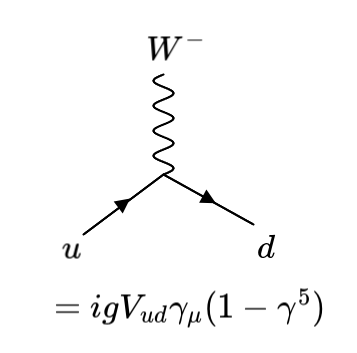
\includegraphics[width=0.4\linewidth]{figs/46a.png}
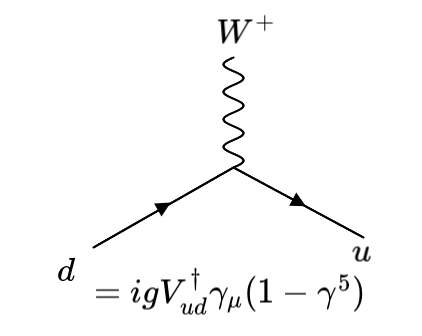
\includegraphics[width=0.4\linewidth]{figs/46b.png}
\end{itemize}
%
\subsection{Unitarity Triangles}
%
Testing for unitarity is equialent to testing for the condition $VV^\dagger =1$. There are different ways of doing this:
\begin{enumerate}
\item \textbf{Universality tests: }
There are three tests of the form $(V^\dagger V)_{ii}=1$, e.g.
$|V_{ud}|^2 +|V_{us}|^2 +|V_{ub}|^2 = 1$.
\item \textbf{Triangle tests: }
There are six tests of the form $(V^\dagger V)_{ij}=0$ for $i \neq j$, e.g.
$V^*_{ub}V_{ud} + V^*_{cb}V_{cd} + V^*_{tb}V_{td} = 0$. 

This is a triangle because it is a sum of three complex numbers. The diagram on the right shows the different connections between the quark types.
\newline
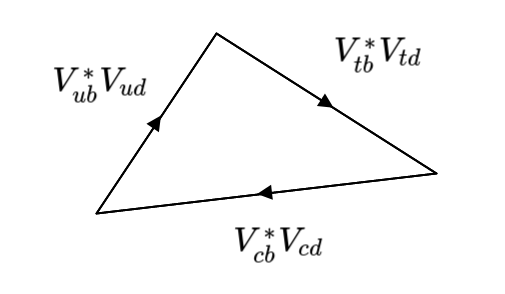
\includegraphics[width=0.6\linewidth]{figs/47a.png}
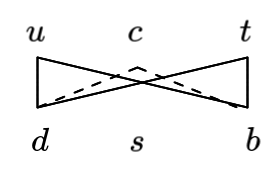
\includegraphics[width=0.3\linewidth]{figs/47b.png}
\end{enumerate}
\textbf{Determining $|V_{ij}|$: }
\begin{itemize}
\item The top left part of $V$ (which doesn't involve $t$ or $b$ quarks) is determined by measuring $\theta_c$ as above. More specifically: $|V_{ud}|$ is determined through $\beta$ and pion decay, $|V_{us}|$ through kaon and tau decays, and $|V_{cd}|$ and $|V_{cs}|$ are determined through $D$ semileptonic decays such as $D \to \pi l \nu$ and $D \to K l \nu$.
\item Additional elements involving the $b$ quark but not the $t$ quark (i.e. "B physics") are determined by $B$ semileptonic decays such as $B \to \pi l \nu$ and $B \to D l \nu$. 
\item $|V_{tb}|$ is determined through single top producgion $t \to bW$, but $|V_{ts}|$ and $|V_{td}|$ are very hard to measure directly. We can use corrections to loop calculations to find these (see later).
\end{itemize}
The results of the combined fits are usefully summarised by the Wolfenstein parametrisation (1983):
\begin{equation}
V = \begin{pmatrix}
1-\frac{\lambda^2}{2} & \lambda & A\lambda^3(\rho - i\eta) \\
-\lambda &  1-\frac{\lambda^2}{2} & A \lambda^2\\
A\lambda^3(1-\rho-i\eta) & -A\lambda^2 & 1 
\end{pmatrix} + \mathcal{O}(\lambda^4),
\end{equation}
where $\lambda \approx \sin\theta_c \approx\ 0.225$, $A \approx\ 0.8$, $\rho \approx\ 0.12$ and $\eta \approx 0.36$ are $\mathcal{O}(1)$. Since $\lambda \gg \lambda^2 \gg \lambda^3$, this expresses a curious hierarchy of the off-diagonal elements, which is not understood! 

Considering the various universality tests and triangles, we can see that in this parametrisation $V$ is unitary.
%
\subsection{CP Violation}
%
Up until now, every term in the electroweak Lagrangian has been CP invariant. In particular, under CP $W_\mu^+ \to - W^{\mu -}$, so that the charged current interaction for leptons transforms as 
\begin{equation}
\begin{split}
\frac{g}{\sqrt{2}}(W_\mu^+\bar{\psi}_LT^-\gamma^\mu \psi_L + W_\mu^-\bar{\psi}_L T^+ \gamma^\mu \psi_L) &\to \frac{g}{\sqrt{2}}(-W^{\mu -}(-\bar{\psi}_L(T^-)^T \gamma_\mu \psi_L) - W^{\mu +}\bar{\psi}_L(T^+)^T \gamma_\mu \psi_L) \\
&= \frac{g}{\sqrt{2}}(W_\mu^- (\bar{\psi}_L T^+ \gamma^\mu \psi_L) + W_\mu^+ \bar{\psi}_L T^- \gamma^\mu \psi_L),
\end{split}
\end{equation}
since $(T^+)^T = T^-$. However, we now need to include the effects of the CKM matrix in the charged-current interaction for quarks:
\begin{equation}
\begin{split}
&\frac{g}{\sqrt{2}}(W_\mu^+\bar{d}_L\gamma^\mu V^\dagger u_L + W_\mu^-\bar{u}_L \gamma^\mu  V d_L)\\
= &\frac{g}{\sqrt{2}}(W_\mu^+\bar{Q}_L T^-\gamma^\mu V^\dagger Q_L + W_\mu^- \bar{Q}_L T^+ \gamma^\mu V Q_L)\\
\to &\frac{g}{\sqrt{2}}(W_\mu^-\bar{Q}_L (T^-)^T\gamma^\mu (V^\dagger)^T Q_L + W_\mu^+ \bar{Q}_L (T^+)^T \gamma^\mu V^T Q_L)\\
= &\frac{g}{\sqrt{2}}(W_\mu^+\bar{Q}_L T^-\gamma^\mu V^{*\dagger} Q_L + W_\mu^- \bar{Q}_L T^+ \gamma^\mu V^* Q_L).
\end{split}
\end{equation}
So we have CP invariance only if $V = V^*$. This means that the electroweak sector is CP invariant for two generations ($N=2$), but not for three generations ($N=3$) if $\delta \neq 0$. In other words, this complex phase, $\delta$, is CP-violating. Note that from the CPT theorem, which states invariance of CPT, that CP violation implies T violation. T is equivalent to complex conjugation, i.e. $\exp(iHt) \to \exp(-iHt)$.

A useful measure of the amount of CP violation is given by the area of the unitarity triangle. For example, if we consider the $bd$ triangle,
\newline
\begin{wrapfigure}{l}{0.4\linewidth}
  \centering
  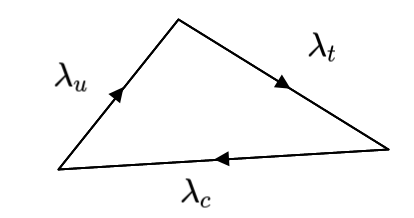
\includegraphics[width=\linewidth]{figs/48a.png}
\end{wrapfigure}
where we have defined $\lambda_i = V_{ib}^* V_{id} = \lambda_i^1 + i \lambda_i^2$. The total area of the triangle is given by
\begin{equation}
\begin{split}
A &= \frac{1}{2}|\underline{\lambda}_u \wedge \underline{\lambda}_c| \\
&= \frac{1}{2}|\lambda_u^1 \lambda_c^2 - \lambda_u^2 \lambda_c^1| \\
&=\frac{1}{2}|\Im(\lambda_u^* \lambda_c)| \\
&= \frac{1}{2}|\Im(V_{ub}V^*_{ud} V_{cb} V^*_{cd})|.
\end{split}
\end{equation}
In fact, all the triangles have the same area (\textit{Exercise:} prove this). We can thus define the \textit{Jarlskog invariant} (Jarlskog, 1983) as
\begin{equation}
\begin{split}
J &= |\Im(V_{ik}V^*_{jk}V_{il}V^*_{jl})| \qquad \text{no sum, } i\neq j \neq k \neq l \\
&=c_1s_1c_2^2s_2c_3s_3\sin\delta \\
&\approx A^2\lambda^6\eta \qquad  \qquad  \qquad \text{in the Wolfenstein parametrisation}.
\end{split}
\end{equation}
For $J=0$, there is no CP violation. Even though $\delta$ is large, CP violation is very small, as $\lambda^6 \approx 0.0001$. It is very difficult to get CP violation. You need:
\begin{itemize}
\item $\delta \neq 0,\ \frac{\pi}{2}$ complex phase;
\item $\theta_1$, $\theta_2$, $\theta_3$ $\neq 0,\ \frac{\pi}{2}$, no trivial angles (otherwise you can rotate the phase away);
\item all masses $\neq 0$, otherwise $N=3$ reduces to $N=2$ and you can rotate the phase away;
\item the masses must be different between up-type and down-type quarks, otherwise $N=3$ reduces to $N=2$ and you can rotate the phase away;
\item at least two interfering amplitudes (because physics $\sim |\mathcal{M}|^2)$;
\item a flavour changing loop, involving all three generations.
\end{itemize}
%
\subsection{$K-\bar{K}$ Mixing and Decay}
%
Remarkably, CP violation was observed already in 1964 (Cronin \& Fitch) through study of decays of neutral $K$ mesons, $K^0=(d\bar{s})$ and $\bar{K}^0=(s\bar{d})$. (CP violation has also been observed in B physics in 2001.) Under CP, $K^0 \leftrightarrow \bar{K}^0$, conventially written as:
\begin{equation}
CP|K^0\rangle = -|\bar{K}^0 \rangle, \qquad CP|\bar{K}^0 \rangle = -|K^0\rangle.
\end{equation}
The CP eigenstates are
\begin{equation}
|K_1\rangle = \frac{1}{\sqrt{2}}(|K^0\rangle - |\bar{K}^0\rangle), \qquad |K_2\rangle = \frac{1}{\sqrt{2}}(|K^0\rangle + |\bar{K}^0\rangle),
\end{equation}
with eigenvalues $+1$ and $-1$ respectively. Kaons decay to combinations of pions:
\begin{equation}
\begin{split}
|\pi^0\pi^0\rangle\ \text{and} \ |\pi^+\pi^-\rangle \qquad &\text{with }CP=+1, \\
|\pi^0\pi^0\pi^0\rangle\ \text{and} \ |\pi^+\pi^-\pi^0\rangle \qquad &\text{with }CP=-1,
\end{split}
\end{equation}
because the pion has odd parity. So if there is no CP violation, $K_1 \to \pi\pi$ and $K_2 \to \pi\pi\pi$. The two pion state has a large phase space so the decay is quick. Converseley, the three pion state has a smaller phase space and the decay is slow ($m_K \approx 495$ MeV whilst $m_\pi \approx 140$ MeV. In reality, there are two \textit{physical} states, which we can observe: $K_S$ ("$K$-short") and $K_L$ ("$K$-long"). Usually, these correspond to 
\begin{equation}
\begin{split}
K_S \to \pi\pi \qquad \textit{i.e. } &K_S \approx K_1, \\
K_L \to \pi\pi\pi \qquad \textit{i.e. } &K_L \approx K_2.
\end{split}
\end{equation}
However, sometimes $K_L \to 2\pi$ and $K_S \to 3\pi$:
\begin{equation}
\eta_{+-} = \frac{\langle\pi^+\pi^-|\mathcal{H}|K_L\rangle}{\langle \pi^+\pi^- |\mathcal{H}|K_S \rangle}, \qquad 
\eta_{00} = \frac{\langle\pi^0\pi^0|\mathcal{H}|K_L\rangle}{\langle \pi^0\pi^0 |\mathcal{H}|K_S \rangle},
\end{equation}
and $\eta_{00} \sim \eta_{+-} \sim 10^{-3}$. Clearly this violates CP. There are two possibilities to explain the observation:
\begin{enumerate}
\item \textbf{Direct CP Violation: }

$K_S,\ K_L$ are CP eigenstates, but the decay process is CP violating.
\begin{figure}[H]
  \subfloat[$\Delta S =1,\ CP$]{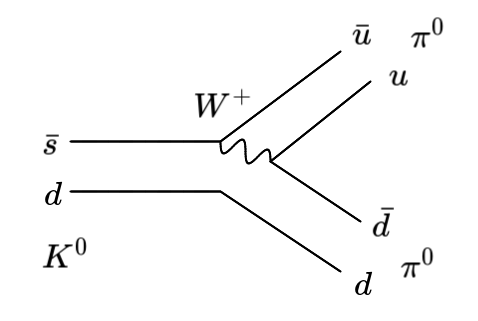
\includegraphics[width=0.5\textwidth]{figs/49a.png}}
  \hfill
  \subfloat[$\Delta S =1, \ CP$ violating if $J\neq 0$]{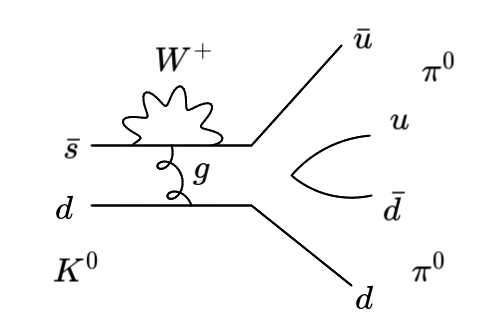
\includegraphics[width=0.5\textwidth]{figs/49b.png}}
  \end{figure}
\item \textbf{Indirect CP Violation: }

$K_S$ and $K_L$ are mixtures of $K_1$ and $K_2$, through interactions given by box diagrams. 
\begin{figure}[H] 
  \subfloat[$\Delta S =2,\ CP$ violating if  $J\neq 0$]{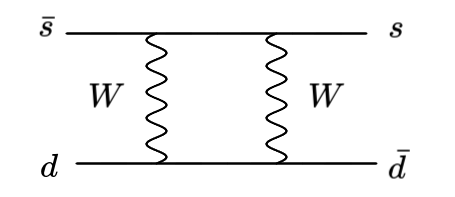
\includegraphics[width=0.5\textwidth]{figs/49c.png}\label{boxdiags1}}
  \hfill
  \subfloat[$\Delta S =2,\ CP$ violating if  $J\neq 0$]{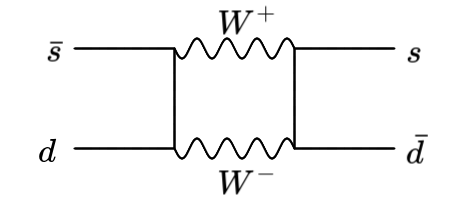
\includegraphics[width=0.5\textwidth]{figs/49d.png}\label{boxdiags2}}
  \end{figure}
\end{enumerate}
Let's focus on indirect CP violation, via kaon mixing. From the CPT theorem,
\begin{equation}
\begin{split}
&\langle K^0 | \mathcal{H} | K^0 \rangle = \langle \bar{K^0} | \mathcal{H} | \bar{K^0} \rangle \\
&\langle K^0 | \mathcal{H} | \bar{K^0} \rangle = \langle \bar{K^0} | \mathcal{H} | K^0 \rangle,
\end{split}
\end{equation}
where the first line is determined by QCD and the second line is determined by electroweak for $\Delta S = 2$. We can write the mass matrix
\begin{equation}
\begin{pmatrix}
M & M_X \\
M_X^* & M 
\end{pmatrix},
\qquad |M_X| \ll M \equiv m_K,
\end{equation}
where $m_K \sim 495$ MeV is the mass of the kaon. The matrix is hermitian so has real eienvalues $M \pm |M_X|$, with eigenvectors
\begin{equation}
\frac{1}{\sqrt{2}} (e^{i\frac{\phi}{2}}|K^0\rangle \pm e^{-i\frac{\phi}{2}}|\bar{K^0}\rangle),
\end{equation}
where $M_X = |M_X|e^{i\phi}$. 

So if there is no CP violation, then $\phi=0$, which means: $|K_L\rangle = |K_2\rangle$ with mass $M+|M_X|$, and $|K_S\rangle = |K_1\rangle$ with mass $M-|M_X|$. We can write $\Delta m_K = m_{K_L} - m_{K_S} = 2|M_X| = 2 \Re M_X$.

If there is CP violation, then $\phi\neq 0$, but we assume it is small. Then we can write
\begin{equation}
\begin{split}
|K_L\rangle &= |K_2\rangle + \frac{i\phi}{2}|K_1\rangle \\
|K_S\rangle &= |K_1\rangle + \frac{i\phi}{2}|K_2\rangle,
\end{split}
\end{equation}
so $|K_L\rangle$ has an admixture of $|K_1\rangle$, and can therefore decay to $\pi\pi$. We can define the parameter $\epsilon$ as a measure of indirect CP violation:
\begin{equation}
\epsilon = \frac{i\phi}{2} = \frac{i\Im M_X}{2\Re M_X} = \frac{i\Im M_X}{\Delta m_K}.
\end{equation}
\subsubsection{Notes:}
\begin{itemize}
\item This analysis is \textit{very} oversimplified! In practice we need to account also for the width $\Gamma$, so $M\to M + \frac{i\Gamma}{2}$, making things rather more complicated. In this case we find
\begin{equation}
\epsilon \approx e^{i\theta_\epsilon}\sin\theta_\epsilon \frac{\Im M_X}{\Delta m_K}, \qquad \tan\theta_\epsilon = \frac{2\Delta m_K}{\Gamma_s - \Gamma_L}, \qquad \theta_\epsilon \approx 45 \degree.
\end{equation}
\item We can compute $M_X$, and thus $\Delta m_K$ and $\epsilon$, from the box diagram:
\begin{equation}
M_X = \frac{\langle K^0 | \mathcal{H} | \bar{K}^0 \rangle}{2m_K},
\end{equation}
where the denominator is a normalisation factor due to density of state arguments (see the QFT course from last term). Calculating the phase of $\epsilon$, and the equivalent parameter $\epsilon^\prime$ from \textit{direct} CP violation is rather harder.
\item In B physics, direct CP violation is more important.
\end{itemize}
%
\subsection{Box Diagrams}
%
As an example, let's revisit one of the box diagrams we saw before.
\newline
  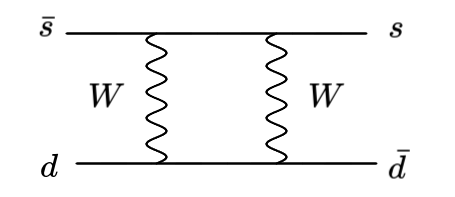
\includegraphics[width=0.6\linewidth]{figs/49c.png}
\newline
We consider the incoming momenta $p=0$ (because we want to calculate the mass). We will work in the Feynman-'t Hooft gauge, so we will also need to consider the three Goldstone boson contributions.
\newline
  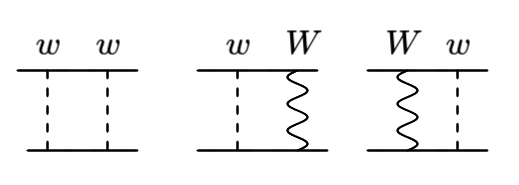
\includegraphics[width=0.6\linewidth]{figs/51a.png}
\newline
The matrix element for the $WW$ diagram can be written:
\begin{equation}
\begin{split}
\mathcal{M}_{WW} = &\sum_{a=u,c,t;\ b=\bar{u},\bar{c},\bar{t}} \bigg(\frac{-ig}{\sqrt{2}}\bigg)^4 V_{as}V_{ad}^* V^*_{bd}V_{bs} \int \frac{d^4l}{(2\pi)^4}\frac{i^4}{(l^2-m_W^2)^2(l^2-m_a^2)(l^2-m_b^2)} \\
&\times \bar{u}_d \gamma^\mu\frac{1}{2}(1-\gamma^5)(\slashed{l}+m_a)\gamma^\nu \frac{1}{2}(1-\gamma^5) u_s \bar{v}_d \gamma_\nu \frac{1}{2}(1-\gamma^5)(-\slashed{l}+m_b)\gamma_\mu \frac{1}{2}(1-\gamma^5)v_s.
\end{split}
\end{equation}
Defining $\xi_a = V_{as}V_{ad}^*$ and ignoring quark masses in the numerator,
\begin{equation}
\begin{split}
\mathcal{M}_{WW} = -&\sum_{a,b} \frac{g^4}{16} \xi_a \xi_b \bar{u}_d \gamma^\mu \gamma^\alpha \gamma^\nu (1-\gamma^5) u_s \bar{v}_d \gamma_\nu \gamma_\beta \gamma_\mu(1-\gamma^5)v_s \\
&\times \int \frac{d^4l}{(2\pi^4)} \frac{l_\alpha l^\beta}{(l^2-m_W^2)^2(l^2-m_a^2)(l^2-m_b^2)}. 
\end{split}
\end{equation}
We can use the identity (\textit{exercise}) 
\begin{equation}
\bar{u}_d \gamma^\mu \gamma^\alpha \gamma^\nu (1-\gamma^5) u_s \bar{v}_d \gamma_\nu \gamma_\beta \gamma_\mu(1-\gamma^5)v_s = 4 \bar{u}_d \gamma^\alpha (1-\gamma^5)u_s \bar{v}_d \gamma_\beta (1-\gamma^5)v_s.
\end{equation}
Note also that the integral is convergent, so Wick rotating the loop momentum $l \to \tilde{l}$, where $l^2 = -\tilde{l}^2$, we get $l_\alpha l^\beta \to \frac{1}{4}\eta^\alpha_\beta \tilde{l}^2$ and $d^4l \to d\Omega_4 i \tilde{l}^2\frac{1}{2}d\tilde{l}^2$. For clarity, we make the substitutions $z=\frac{\tilde{l}^2}{m_W^2}$, $x_a = \frac{m_a^2}{m_W^2}$, $x_b = \frac{m_b^2}{m_W}^2$. This leads to
\begin{equation}
\begin{split}
\mathcal{M}_{WW} = +&\sum_{a,b} \frac{iG_F^2}{16\pi^2} \xi_a \xi_b^*\ 2\bar{u}_d \gamma^\mu (1-\gamma^5) u_s \bar{v}_d \gamma_\mu (1-\gamma^5) v_s m_W^2 \\
&\times \int_0^\infty dz \frac{z^2}{(z+1)^2(z+x_a)(z+x_b)} \\
\equiv +&\sum_{a,b} \frac{iG_F^2}{16\pi^2} \xi_a \xi_b^*\ Q_K^t \mathcal{I}_2(x_a,x_b).
\end{split}
\end{equation}
You can evaluate the other three diagrams in the same way (\textit{exercise}). You find
\begin{equation}
\begin{split}
\mathcal{M} &= \mathcal{M}_{WW} + \mathcal{M}_{ww} + 2\mathcal{M}_{Ww} \\
&= \sum_{a,b} \frac{iG_F^2}{16\pi^2} \xi_a \xi_b^* Q_K^t\bigg((1+\frac{1}{4}x_a x_b)\mathcal{I}_2(x_a,x_b) + 2x_a x_b \mathcal{I}_1(x_a,x_b) \bigg),
\end{split}
\end{equation}
where 
\begin{equation}
\mathcal{I}_1(x_a,x_b) = \int_0^\infty dz \frac{z}{(z+1)^2(z+x_a)(z+x_b)}.
\end{equation}
Note that $\mathcal{M}$ vanishes if we ignore the quark masses, because $\sum_a \xi_a =0$, by the unitarity triangle. The integrals can be evaluated using partial fractions (\textit{exercise}), e.g.
\begin{equation}
\begin{split}
&\mathcal{I}_k(x_a,x_b) = \frac{A_k(x_a)-A_k(x_b)}{x_a-x_b}; \\
\text{where } \qquad &A_1(x) = -\bigg(\frac{1}{1-x} + \frac{x \ln x}{(1-x)^2}\bigg), \qquad A_2(x) = \frac{1}{1-x} + \frac{x^2 \ln x}{(1-x)^2}.
\end{split}
\end{equation}
Since the process is non-leptonic, we have trouble with the matrix elements: we need
\begin{equation}
\begin{split}
&\langle K^0 | (\bar{d}\gamma^\mu (1-\gamma^5)s)^2| \bar{K}^0 \rangle \\
= &\sum_X 2 \langle K^0 | \bar{d}_i \gamma^\mu (1-\gamma^5) s_i | X \rangle \langle X| \bar{d}_j \gamma_\mu (1-\gamma^5) s_j | \bar{K}^0 \rangle \\
&+\sum_X 2 \langle K^0 | \bar{d}_i \gamma^\mu (1-\gamma^5) s_j | X \rangle \langle X| \bar{d}_j \gamma_\mu (1-\gamma^5) s_i | \bar{K}^0 \rangle,
\end{split}
\end{equation}
where $i,j$ label colour and we have inserted a complete set of states $X$. Note that this includes contributions from both box graphs: the first term corresponds to Fig. \ref{boxdiags2}, and the second term corresponds to Fig. \ref{boxdiags1}.

In order to proceed further, we make the "vacuum saturation" approximation, which consists of sending $|X\rangle \langle X| \to |0 \rangle \langle 0|$. We hope that this makes up the most significant contribution. We can write
\begin{equation}
\langle 0 | \bar{d}_i \gamma_\mu (1-\gamma^5)s_j | \bar{K}^0 \rangle = i p_\mu \frac{1}{3} \delta_{ij} f_K,
\end{equation}
where $f_K$ is the Kaon decay constant. This means we can approximate
\begin{equation}
\langle K^0 | (\bar{d}\gamma^\mu (1-\gamma^5)s)^2| \bar{K}^0 \rangle \approx \frac{2}{9} m_K^2 f_K^2 (\delta_{ii}\delta_{jj} + \delta_{ij}\delta_{ij}) = \frac{8}{3}m_K^2 f_K^2.
\end{equation}
To account for the fact we made the vacuum stauration approximation, we introduce a "fudge factor" $B_K$. From lattice calculations, this has been determined as $B_K \approx 0.8$. So all in all,
\begin{equation}
\langle K^0 | \mathcal{H} | \overline{K}^0 \rangle = \frac{G_f^2 m_W^2}{16\pi^2} \frac{8}{3}m_K^2 f_K^2 B_K \sum_{ab} \xi_a \xi_b \bigg( (1+\frac{1}{4} x_a x_b) \mathcal{I}_2 + 2 x_a x_b \mathcal{I}_1\bigg).
\end{equation}
We need to compute $\sum_{ab}\xi_a \xi_b^* F_{ab}$, where $F_{ab}$ is equivalent to the bracketed term in the above equation. First we note that $\xi_u = -\xi_c -\xi_t$, from the unitarity triangle, so
\begin{equation}
\sum_{ab} \xi_a \xi^*_b F_{ab} = \xi_c^2(F_{cc} + F_{uu} - 2F_{uc}) + 2 \xi_c \xi_t (F_{ct} - F_{ut} + F_{uu} - F_{uc}) + 3 \xi_t^2(F_{tt} + F_{uu} - 2 F_{ut}).
\end{equation}
Now, $x_u \ll x_c \ll 1$, $x_t >1$. As an exercise, you can show that $F_{uu} \approx 1$, $F_{uc} \approx 1 + x_c \ln x_c + x_c$,  $F_{cc} \approx 1 + 2x_c \ln x_c + 3x_c$: so $F_{cc} + F_{uu} -2F_{uc} \approx x_c$, etc. Using the Wolfenstein parametrisation:
\begin{equation}
\begin{split}
\xi_c = V_{cs}V_{cd}^* = \bigg(1-\frac{\lambda^2}{2}\bigg)(-\lambda), \\
\xi_t = V_{ts}V_{td}^* = (-A\lambda^2)A\lambda^3(1-\rho+i\eta).
\end{split}
\end{equation}
So 
\begin{itemize}
\item the $\xi_c^2$ term is $\mathcal{O}(m_c^2)O(\lambda^2) \sim 2 \times 10^{-5}$: largest, but no CP violation,
\item the $2\xi_c \xi_t$ term is $\mathcal{O}(m_c^2)\mathcal{O}(\lambda^6) \sim 1 \times 10^{-7}$,
\item the $\xi_t^2$ term is $\mathcal{O}(m_t^2)O(\lambda^10) \sim 2 \times 10^{-6}$: the largest CP violating term, because $m_t$ is so large.
\end{itemize}
So 
\begin{equation}
\begin{split}
\Delta m_K = 2\frac{|\langle K^0|\mathcal{H}|\bar{K}^0\rangle |}{2m_K}&= 2M_X \\ &\approx \frac{G_F^2}{6\pi^2}m_K f_K^2 B_K\sin^2\theta_c m_c^2 \\
&\sim 3\times 10^{-5} \text{ GeV}.
\end{split}
\end{equation}
Experimentally, this is measured to be $3.5 \times 10^{-6}$ eV. This calculation was used by GIM in 1970 to predict the charm mass, $m_c \sim 1.5$ GeV. 

Now looking at the CP violating terms, the dominant contribution is $\xi_t^2$. Define
\begin{equation}
E_{tt} \equiv F_{tt} + F_{uu} - 2F_{ut} = + \frac{3}{2} \frac{x_t^3 \ln x_t}{(x_t-1)^3} + \frac{x_t^3 - 11x_t^2 + 4x_t}{4(x_t-1)^2},
\end{equation}
known as the Inami-Lim function (1981). We know that
\begin{equation}
\Im \xi_t^2 = 2\Im \xi_t \Re \xi_+ = -2A^4 \lambda^{10}(1-\rho)\eta,
\end{equation}
so
\begin{equation}
\begin{split}
\Re \epsilon &= \frac{\Im M_X}{2 \Delta m_K} = \frac{2 A^4 \lambda^{10}(1-\rho)\eta}{4\lambda^2 x_t} E_{tt}\\
&= \frac{1}{2} A^4 \lambda^8 (1-\rho) \eta x_c^{-1} E_{tt} \\
&\approx 3\times 10^{-3}.
\end{split}
\end{equation}
Experimentally, this was measured as 1.5$\times 10^{-3}$. So this is indeed the origin of CP violation in $K-\bar{K}$ mixing! Note that a heavy top is essential. The most remarkable facet is that a top quark of mass 175 GeV gives CP violation in $K-\bar{K}$, which has a natural scale of $\Delta m_K$: an effect crossing over 17 orders of magnitude!
%
\subsection{Neutrinos}
%
So far we have assumed $m_\nu \equiv 0$. Indeed, no neutrino mass has yet been measured, and we have limits $m_\nu \leq 0.3$ eV. However, neutrinos are observed to "oscillate", or "mix":
\begin{itemize}
\item atmospheric neutrions undergo processes like $\pi^- \to \mu^- \bar{\nu}_\mu \to e^- \nu_e \nu_\mu \bar{\nu}_\mu$, interchanging $\nu_e$ and $\nu_\mu$. These oscillations were observed by Kamiokande in 1998;
\item solar neutrinos are produced during $\beta$-decay to $\nu_e$, but $\nu_\mu$ and $\nu_\tau$ have also been seen, at Sudbury in the early 2000s;
\item reactor neutrinos are now observed at many experiments, where neutrino beams can be viewed in the lab.
\end{itemize}
Mixing naturally arises through the presence of mass terms. The easiest way to include such terms in electroweak theory is through Yukawa terms, just like for quarks.
\begin{equation}
\mathcal{L}^L_{Y} = - \bigg(Y_{ij}^e \bar{L}_L^i \phi e_R^j + h.c. \bigg) - \bigg(Y_{ij}^\nu \bar{L}_L^i \phi^c \nu_R^j + h.c. \bigg),
\end{equation}
where the first bracket gives mass to the electrons and the second bracket gives mass to the neutrinos. Note that:
\begin{equation}
\begin{split}
L_L = &\begin{pmatrix} \nu_{eL} \\ e_L \end{pmatrix}, 
\begin{pmatrix} \nu_{\mu L} \\ \mu_L \end{pmatrix},
\begin{pmatrix} \nu_{\tau L} \\ \tau_L \end{pmatrix}
\qquad Y=-\frac{1}{2} \ \text{as before}; \\
&e_R, \mu_R, \tau_R \qquad \qquad \qquad \qquad Y=-1 \ \text{as before}; \\
&\nu_{eR}, \nu_{\mu R}, \nu_{\tau R}\qquad \qquad \qquad Y=0\ \text{new: need } Y=0 \text{ because } Q=0.
\end{split}
\end{equation}
This works because the complex doublet $\phi$ has $Y=+\frac{1}{2}$ and $\phi^c$ has $Y=-\frac{1}{2}$.  As for quarks, we can rotate into the mass basis. The mass terms are then
\begin{equation}
-\sum_{l=e, \mu\,\tau} m_l \bar{l}l\ - \sum_{\nu=\nu_e,\nu_\mu, \nu_\tau} m_\nu \bar{\nu}\nu,
\end{equation}
but the charged current becomes
\begin{equation}
\frac{1}{2}J_\mu^l = \sum_i \bar{\nu}_L^i \gamma_\mu e_L^i \to \sum_{ij} \bar{\nu}_L^i \gamma_\mu U^{ij}e_L^j,
\end{equation}
where $U$ is the PMNS matrix, developed by Pontecorvo and Maki (1957), and Nakagawa and Sakata (1962). The $\bar{\nu}_L^i$ terms are changed from being flavour eigenstates to being mass eigenstates.

There are three mixing angles (now all measured) and a CP violating phase (not yet measured).
\subsubsection{Notes}
\begin{itemize}
\item It is usual to attach the mixing to "up-type" leptons, i.e. the neutrinos. This is the opposite of what we did for quarks, and is down to historical convention.
\item It is usual to use the flavour basis (where the charged current is diagonal and mixing is in the masses) rather than the mass basis (where mixing is in the charged current, and the masses are diagonal). Again, this is historical: the neutrino flavour is labelled due to production and measurement, whereas the masses are still not yet measured.
\item Because the masses are only observed via mixing, we can so far only observe mass differences. These are $\Delta m_{12} \approx 10^{-2}$ eV between the first and second generations, and $\Delta m_{13} \approx \Delta m_{23} \approx 0.05$ eV between the first and third and second and third generations. Remember that $m_e =0.5$ MeV, which is $10^8$ times larger.
\end{itemize}
\subsection{Majorana Masses}
We call $\nu_R$ a "sterile" neutrino, in that it has no quantum numbers (except lepton number), so it can only be seen due to a mass, i.e. through neutrino mixing. We can use the charge conjugation operator $C=i \gamma^2 \gamma^0$, to define $\nu_R^C = C\bar{\nu}_R^T$, $\bar{\nu}_R^C = \nu_R^T C$, and write down a "Majorana mass term":
\begin{equation}
-\frac{M}{2}\bigg( \bar{\nu}_R^C \nu_R + \bar{\nu}_R \nu_R^C \bigg) = -M \nu_R^T C \nu_R.
\end{equation}
This is Lorentz invariant and also SU(2)$_L \otimes$U(1)$_Y$ invariant, because $\nu_R$ is a singlet. However, it explicitly violates lepton number. If there are both Dirac and Majorana masses present, we have terms
\begin{equation}
\sim -m(\bar{\nu}_L\nu_R + \bar{\nu}_R \nu_L) - M \nu_R^C \nu_R,
\end{equation}
so the mass matrix is of the form
\begin{equation}
\begin{pmatrix}
0 & m \\
m & M
\end{pmatrix},
\end{equation}
with eigenvalues
\begin{equation}
\frac{M}{2} \pm \frac{1}{2} \sqrt{M^2 + 4m^2}.
\end{equation}
So for $M \gg m$, we have masses $M$ and $\frac{m^2}{M} \ll m$. This is called the "see-saw mechanism". For example, if $M \sim 10^{19}$ GeV at the Plank scale, and $m \sim 100$ GeV at the electroweak scale, then $\frac{m^2}{M} \sim 10^{-6}$ eV, which is very small.

If we include a Majorana mass term like this we get two extra CP violating phases in the PMNS matrix, which can no longer be roatated away. This could be how nature works, but there are many other possibilities. 
\subsection{Baryogenesis}
To create matter (i.e. baryons) in the early universe, we need (Sakharov, 1967):
\begin{itemize}
\item B-violating processes. These could be due to anomalies in electroweak physics, but are the effects too small?;
\item CP-violating processes, to create matter-antimatter asymmetry. These could be due to the CKM matrix in electroweak physics, but again are the effects too small?;
\item A first order phase transition, in order to avoid washing out the asymmetry. This could be from spontaneous symmetry breaking in electroweak physics, but this is only first order for $m_h < 70$ GeV, and experimentally $m_h = 125$ GeV.
\end{itemize}
In other words, electroweak theory almost needs all three of these conditions, but not quite. There are many alternatives, one of which is leptogenesis, which uses CP-violation in the lepton sector along with Majorana mass terms.